\setcounter{chapter}{0}
\chapter{Presentation of the Host Organization: Algérie Télécom}
\label{chap:presentation}

\section{History}
\label{subsec:historique}

Algérie Télécom is the leader in the rapidly growing Algerian telecommunications market. It offers a complete range of voice and data services to residential and professional clients. Algérie Télécom is a publicly owned joint-stock company operating in the electronic communications networks and services market. Its creation was formalized by Law 2000/03 of August 5, 2000, establishing the general rules relating to postal and telecommunications services, as well as the resolutions of the National Council for State Participations (CNPE) of March 1, 2001, creating a Public Economic Enterprise named "Algérie Télécom". Algérie Télécom is therefore governed by this law, which grants it the status of a public economic enterprise in the legal form of a joint-stock company (SPA) with a share capital of 50,000,000,000 Dinars, registered in the trade register center on May 11, 2002. Officially entering into activity on January 1, 2003, it commits to the world of Information and Communication Technologies with three objectives:
\begin{itemize}
    \setlength{\itemsep}{4pt}
    \setlength{\parskip}{4pt}
    \setlength{\parsep}{4pt}
    \item Profitability
    \item Efficiency
    \item Service quality
\end{itemize}

Its ambition is to achieve a high level of technical, economic, and social performance in order to sustainably maintain its leadership in its field, in an increasingly competitive environment. Its concern also consists of preserving and developing its international dimension and participating in the promotion of the information society in Algeria.

\section{Missions and Objectives}
\label{subsec:missions}

\textbf{Major Activity:} Provide telecommunications services enabling the transport and exchange of voice, written messages, digital data, and audiovisual information. Develop, operate, and manage public and private telecommunications networks; establish, operate, and manage interconnections with all network operators.

\textbf{Commitments:} Algérie Télécom is committed to the world of information and communication technologies with the following objectives:
\begin{itemize}
    \item Increase the range of telephone services and facilitate access to telecommunications services for the greatest number of users, particularly in rural areas;
    \item Improve the quality of services offered and the range of services provided, and make telecommunications services more competitive;
    \item Develop a reliable national telecommunications network connected to the information highways.
\end{itemize}

\section{General Organization Chart of Algérie Telecom}
\label{subsec:organisation}

Algérie Telecom is organized into Divisions, Central Directorates, and 60 operational telecommunications directorates (OTD) distributed across the entire national territory, including three in Algiers. Each OTD includes several TCA (Telecommunications Commercial Agency) and MPC (Maintenance and Production Center).

\textbf{Acronyms:}
\begin{itemize}
    \setlength{\itemsep}{4pt}
    \setlength{\parskip}{4pt}
    \setlength{\parsep}{4pt}
    \item CEO: Chief Executive Officer (President Director General)
    \item DGA: Deputy General Director
    \item OTD: Operational Telecommunications Directorate
    \item Div: Division
    \item Dir: Directorate
    \item TCA: Telecommunications Commercial Agency
    \item MPC: Maintenance and Production Center
\end{itemize}

\begin{figure}[H]
\centering
\fbox{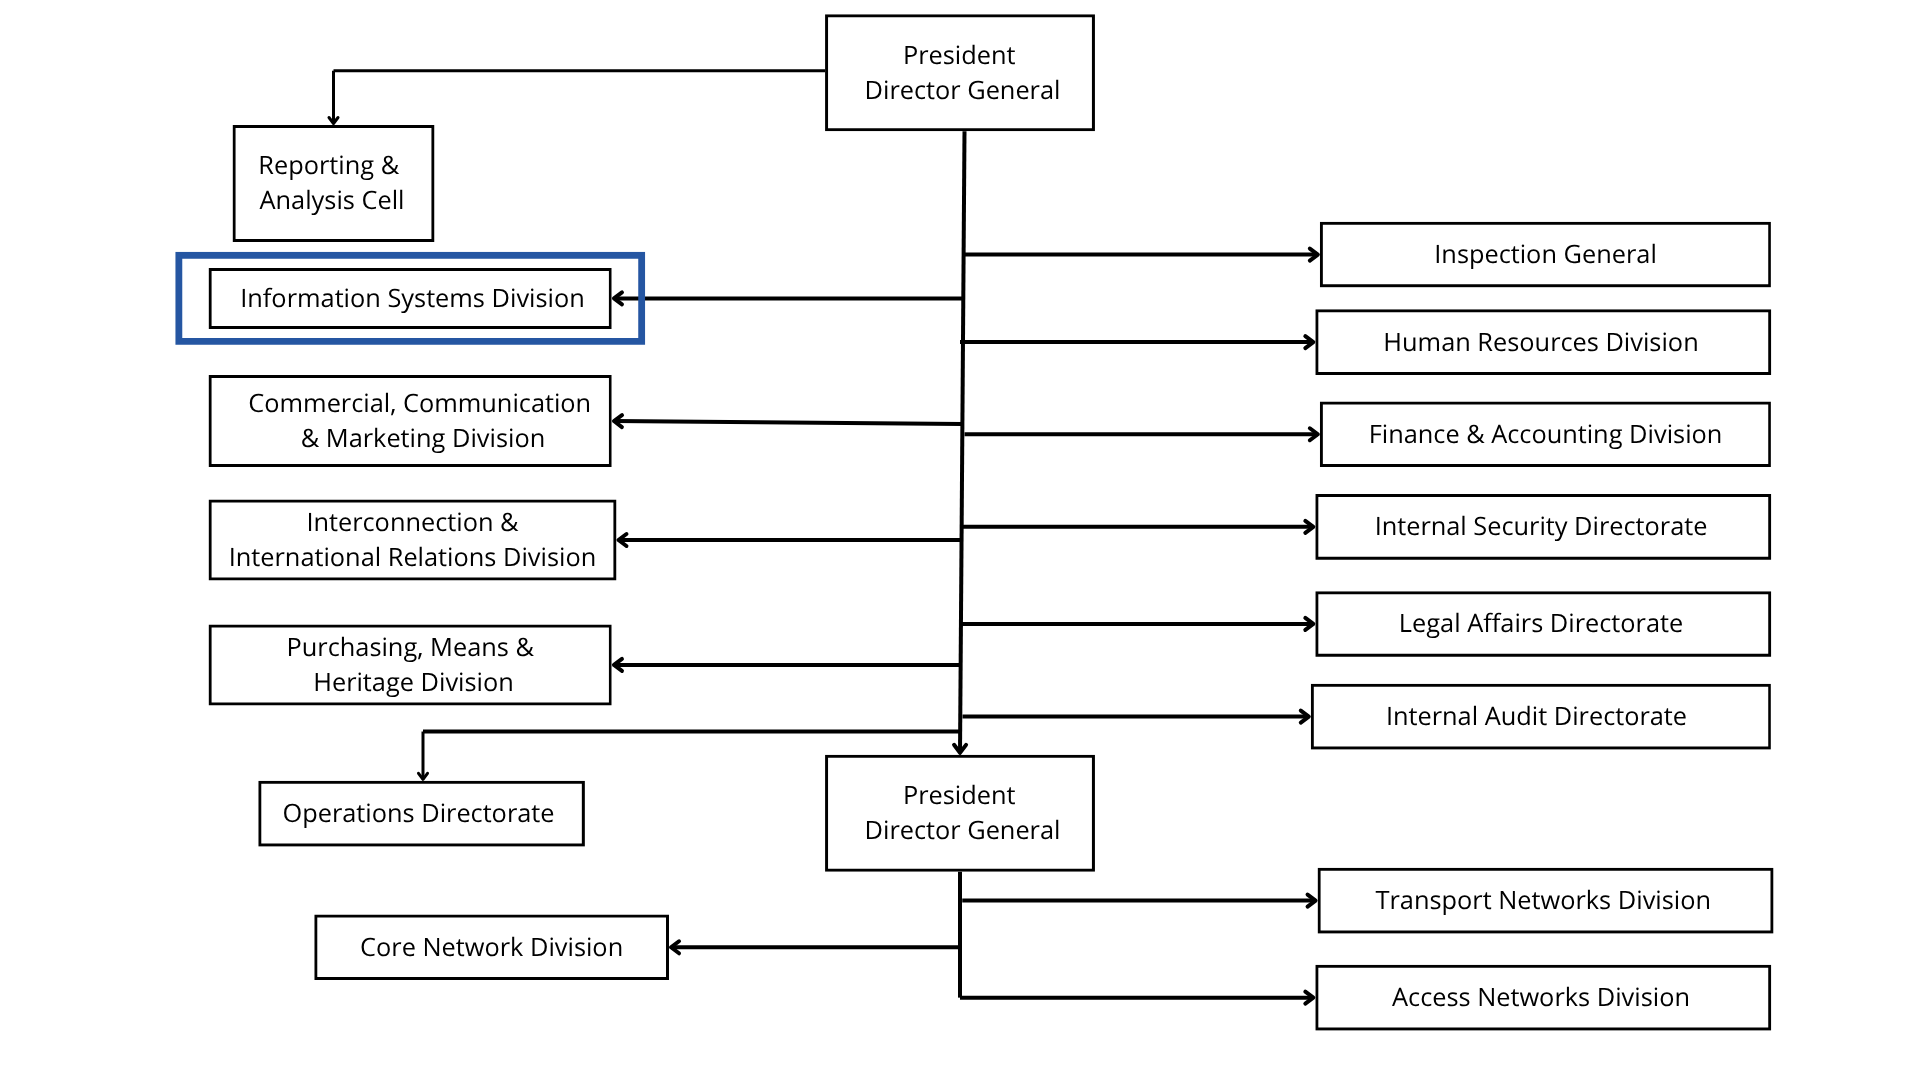
\includegraphics[width=0.8\textwidth]{figs/Director general.png}}
\caption{General Organization Chart of Algérie Telecom}
\label{fig:organigramme_general}
\end{figure}

% ========== 1.2 PRESENTATION OF THE HOST STRUCTURE ==========
\section{Presentation of the Host Structure}
\label{sec:structure_accueil}

\subsection{Presentation of the Supervised Structure (Information Systems Division)}
\label{subsec:dsi}

The Information Systems Division (ISD) of Algérie Telecom is an IT services division, whose mission is to provide the company with cutting-edge information systems covering all its activities.

The Information Systems Division has the following main missions:
\begin{itemize}
    \setlength{\itemsep}{4pt}
    \setlength{\parskip}{4pt}
    \setlength{\parsep}{4pt}
    \item Assess and evolve the company's internal IT infrastructure
    \item Ensure the sustainability of management applications and their integration into the company's overall information system
    \item Provide support to users of the company's information systems and computer equipment (throughout the national territory)
    \item Manage and maintain the company's information fabric, making necessary information available in all its aspects (archiving, databases, portals, as well as technical documents) to the various actors of the organization
    \item Propose solutions and services, in the field of information systems, for internal clients
    \item Establish a center of expertise in information systems
\end{itemize}

\subsection{Organization Chart of the Information Systems Division}
\label{subsec:orga_dsi}

\begin{figure}[H]
\centering
\fbox{
\includegraphics[width=0.8\textwidth]{figs/Division Systemes d'information.png}}
\caption{Organization Chart of the Information Systems Division}
\label{fig:organigramme_dsi}
\end{figure}

\subsection{Strategic Positioning and Prospects}
\label{subsec:positioning}

\subsubsection*{Role in National Digital Transformation}

Algérie Télécom occupies a strategic position within the Algerian digital ecosystem as the essential pillar of the national telecommunications infrastructure. Its role surpasses that of a simple operator, embracing a mission as the catalyst of digital transformation on a national scale. The company provides the critical connectivity required by all sectors of activity.

\subsubsection*{Competitive Advantages}

\begin{itemize}
    \item \textbf{Monopoly on Fixed Infrastructure:} As the historical operator, the company holds the monopoly on fixed-line telephony and fixed Internet, conferring a unique and indispensable position in the national market.
    \item \textbf{Technical Expertise:} The personnel of Algérie Télécom benefit from certifying training with international technology leaders such as Huawei, ensuring a level of technical expertise aligned with global standards.
    \item \textbf{Deep Understanding of the National Market:} As a public enterprise under ministerial supervision, Algérie Télécom possesses a profound understanding of the challenges, constraints, and specific needs of the Algerian market and its public institutions.
\end{itemize}

\subsubsection*{Development Prospects}

Algérie Télécom orients itself toward reinforcing its role as the leader of connectivity in Algeria. Prospects include the development of cloud and data center services, the strengthening of cybersecurity for critical infrastructure, and the accompaniment of public organizations in their transition toward advanced digital operational models.

% ========== 1.3 GENERAL PROJECT FRAMEWORK ==========
\section{General Project Framework}
\label{sec:cadre}

The digital landscape is undergoing a profound transformation. Cyberattacks have seen an alarming increase in recent years, reflecting threats that are increasingly sophisticated, industrialized, and often state-sponsored. In 2024, the number of ransomware victims increased by 29\%. In parallel, the average cost of a data breach reached 4.88 million dollars per incident, a 10\% increase in a single year \cite{ref-cost-breach} \cite{ref-ransomware}.

Faced with this growing threat, enterprises and public institutions have no choice but to equip themselves with a Security Operations Center (SOC), whether internal or externalized through the SOCaaS model. However, for an organization of Algérie Télécom's stature and national responsibility, the challenge extends beyond the mere technical deployment of a security platform. It touches upon a fundamental question of national strategic importance: technological sovereignty.

\subsection{Risk of the Absence of a SOC}
\label{subsec:risque}

The absence of a SOC exposes the organization to major and multifaceted risks.

\textbf{Late Detection of Threats:} Advanced cyberattacks, such as ransomware and Advanced Persistent Threats (APT), can remain invisible for several days, weeks, or even months. This can lead to considerable recovery costs, as well as irreparable damage to the reputation of the institution due to massive data leaks.

\textbf{Poor Reactive Incident Management:} Without a SOC, teams react to incidents only after they have occurred, which considerably extends the mean time to recovery (MTTR). For example, a Distributed Denial of Service (DDoS) attack can cause a critical service interruption lasting over 12 hours before a solution is implemented. This can cause immediate financial losses and a significant weakening of the trust placed by citizens and institutional partners.

\textbf{Regulatory Non-Compliance:} Evolving national and international regulations demand rigorous traceability of security incidents and robust protection of personal and sensitive data. In the absence of a SOC, the organization cannot justify its compliance. This may result in financial penalties, legal sanctions, and exclusion from public procurement processes and strategic national projects.

\subsection{The Strategic Imperative : Digital Sovereignty and the Open-Source Mandate}
\label{subsec:souverainete}

Beyond the operational risks lies an even more fundamental strategic challenge. Algérie Télécom, as the sole national telecommunications operator and a critical pillar of Algeria's digital infrastructure under the supervision of the Ministry of Post and Telecommunications, confronts a profound structural vulnerability: \textbf{technological dependency on foreign proprietary solutions.}

Every modification, every upgrade, every security patch, and every expansion of the national network currently requires engaging with foreign vendors. These vendors control the licensing, dictate the roadmap, and hold the keys to the proprietary technologies deployed within Algeria's most sensitive infrastructure. Every such transaction demands payment in foreign currency, creating a continuous and growing financial drain on the national economy. More critically, the opaque nature of proprietary software means its internal workings cannot be audited. There can be no absolute certainty that backdoors, intentional or otherwise, do not exist within the code that runs the nation's critical communications.

This is not merely a technical inconvenience. It is a \textbf{problem of national sovereignty.}

The global geopolitical landscape has undergone a decisive shift. Nations are increasingly recognizing that technological dependency on foreign powers constitutes an unacceptable strategic vulnerability. The illusion that technology is neutral and that nations can indefinitely entrust their digital foundations to external proprietary systems has been irrevocably shattered.

\begin{comment}
    
\textbf{The case of the French Republic is both instructive and historically significant.} Following a series of political tensions and concrete strategic concerns between France and the United States of America, the French government made a landmark decision: to migrate the entirety of its government computer systems from Microsoft Windows to open-source Linux-based operating systems. This decision was not driven by a mere technical preference or budgetary consideration. It was a \textbf{national security imperative.}

France understood with clarity that:

\begin{itemize}
    \item A foreign power could, in a moment of geopolitical crisis, exert immense pressure by threatening to shut down, restrict access to, or revoke the licenses of the proprietary operating systems upon which the entire functioning of the French state depended.
    \item Dependency on a foreign vendor's closed-source software represents an unacceptable single point of failure for the continuity of government operations, the protection of classified data, and the preservation of national decision-making autonomy.
    \item The only path to true digital resilience and genuine national independence is to \textbf{own and control the entire technology stack} — from the operating system to the application layer.
\end{itemize}

France chose independence. France chose open source. This decision validates what security strategists and government experts globally have come to recognize as a fundamental truth: for critical national infrastructure, open-source solutions are not merely an alternative to proprietary offerings — they represent the \textbf{only strategically sound and responsible choice.}

\end{comment}

Open-source technology delivers precisely what proprietary solutions, by their very nature, cannot guarantee:

\begin{itemize}
    \item \textbf{Full and Sovereign Control:} \hspace{0.2cm} The organization owns the code. It can be modified, extended, and adapted without waiting for the authorization, roadmap, or commercial interests of a foreign vendor. National infrastructure must respond to national priorities, not foreign corporate strategies.
    
    \item \textbf{Complete Auditability and Trust:} \hspace{0.2cm} Every single line of code can be inspected by national experts. There are no hidden functions, no undisclosed backdoors, and no possibility of foreign surveillance embedded within the software. Trust is established through verification, not through contractual assurances from a foreign corporation.
    
    \item \textbf{Cost Sovereignty:} \hspace{0.2cm} Open-source solutions eliminate recurring license fees denominated in foreign currency. The financial investment is redirected toward developing national expertise, training Algerian engineers, and building internal capabilities — investing in the nation's human capital rather than transferring wealth to foreign software corporations.
    
    \item \textbf{Strategic Flexibility:} \hspace{0.2cm} The technology is adapted to the specific needs and constraints of the organization, rather than the organization being forced to adapt its processes and security posture to the limitations of a proprietary product.
    
    \item \textbf{Security Through Radical Transparency:} \hspace{0.2cm} Vulnerabilities in open-source software are discovered and patched by a global community of experts. The organization is not dependent on the security team of a single foreign company, which may have priorities, timelines, and interests that do not align with Algeria's national security requirements.
    
    \item \hspace{0.6cm}\textbf{Operational Resilience and Strategic Autonomy:} There is no vendor lock-in. No foreign entity possesses the ability to remotely disable, restrict, or shut down the nation's critical infrastructure. The continuity of national operations is guaranteed by sovereign national capability, not by the goodwill of a foreign corporation or government.
    
    \item \textbf{Building National Intellectual Capital:} \hspace{0.2cm} Adopting and mastering open-source technologies compels national engineers to understand systems deeply, not merely to operate proprietary black boxes. This cultivates genuine national expertise and builds the foundation for future technological innovation from within the country.
\end{itemize}

For Algérie Télécom, the imperative is clear. As the backbone of Algeria's digital future, the company is called upon to lead a historic transition toward \textbf{technological sovereignty.} This transition entails:

\begin{enumerate}
    \item \textbf{Reducing and progressively eliminating dependency on foreign proprietary solutions} across all layers of the critical national telecommunications infrastructure.
    \item \textbf{Building internal mastery and national expertise} capable of deploying, managing, securing, and evolving open-source systems with complete autonomy.
    \item \textbf{Creating a national reference model} that demonstrates — at the largest scale — the viability, performance, and security of open-source solutions, thereby paving the way for other Algerian institutions and enterprises to follow.
    \item \textbf{Transforming cybersecurity from a service purchased from abroad into a sovereign national capability} that protects Algeria's digital assets with tools and expertise that are fully owned, fully controlled, and fully trusted.
\end{enumerate}

This is not an idealistic aspiration. It is a practical, proven, and urgently necessary strategy that leading nations have already begun to execute. The decision to design and deploy an open-source Security Operations Center and SOC as a Service platform is a concrete, strategic step in this direction. It constitutes a declaration of technological independence and a foundational contribution to the digital sovereignty of the nation.

\subsection{Envisioned Solution and Its Objectives}
\label{subsec:solution}

The organization faces a dual ambition: to strengthen its own internal cybersecurity posture by establishing an internal SOC, while simultaneously creating a SOC as a Service (SOCaaS) offering destined for external clients, particularly small and medium-sized enterprises and organizations with limited resources.

Currently, the absence of an internal SOC exposes the enterprise to the risks previously established. Simultaneously, the SOCaaS market is dominated by costly and rigid proprietary solutions, which opens a window for an innovative offering that is both economically accessible and strategically sovereign.

This project aims to design and deploy a SOC and SOCaaS solution based entirely on open-source technologies, with the objective of providing a cybersecurity infrastructure that is modular, scalable, cost-effective, and fully under sovereign control.

\textbf{SOC as a Service Architecture Design:} Define the SOC architecture, taking into account security requirements, alert management, incident management, and automated response (SOAR). This SOC must be modular, enabling the easy integration of new tools, data sources, and evolving threat intelligence.

\textbf{Implementation of Open-Source Tools:} Deploy open-source tools for the collection, management, and analysis of security logs and alerts. For example: Wazuh for SIEM and XDR capabilities, and Shuffle or TheHive for SOAR orchestration and automation.

\textbf{Automation of Detection and Response:} Implement incident detection rules and define automated response scenarios. This includes the creation of SOAR playbooks for responding to detected threats in real time, reducing the dependency on human intervention for repetitive tasks.

\textbf{Dashboards and Reporting:} Create interactive dashboards and comprehensive reports to monitor the security posture in real time and to conduct thorough post-incident forensic analyses.

\textbf{Performance and Scalability Testing:} Test the SOC platform in a simulated environment with diverse data sources (networks, systems, applications) to evaluate its capacity to manage a high volume of security incidents while ensuring rapid detection and response times.

\textbf{Comprehensive Documentation:} Produce detailed documentation encompassing the description of the architecture, installation procedures, configuration guides, and practical use-case examples to facilitate adoption, operation, and knowledge transfer.

% ========== 1.4 CONCLUSION ==========
\section{Conclusion}
\label{sec:conclusion}

Algérie Télécom represents a major institutional actor in Algeria's digital transformation. Its unique position as the historical telecommunications operator, its extensive national infrastructure covering the entirety of the country, and its public service mission make it a privileged partner for understanding and analyzing the challenges of digitalizing the Algerian public sector.

However, this position of critical national importance also imposes a profound strategic responsibility. In an era of geopolitical uncertainty and increasingly sophisticated cyber threats, the technological choices made by the national operator carry consequences that extend far beyond technical performance metrics. They touch upon the fundamental questions of national sovereignty, strategic autonomy, and the protection of the nation's digital future.

This detailed presentation of the host organization establishes the institutional and technical context necessary for understanding the research work conducted within the framework of this master's thesis. It also articulates the strategic vision that motivates this project: to build, with open-source technologies and sovereign expertise, the cybersecurity infrastructure that Algeria deserves.

% ========== BIBLIOGRAPHY ==========
\begin{thebibliography}{99}
\bibitem{ref-at-creation} Algérie Télécom, \textit{Présentation de l'entreprise}, available at: \url{https://www.algerietelecom.dz}
\bibitem{ref-at-dg} Algérie Télécom, \textit{Mot du Directeur Général}, available at: \url{https://www.algerietelecom.dz}
\bibitem{ref-idoom} Algérie Télécom, \textit{Offres Idoom Fibre}, available at: \url{https://www.algerietelecom.dz}
\bibitem{ref-comintal} Algérie Télécom, \textit{Filiales du Groupe Télécom Algérie}, available at: \url{https://www.algerietelecom.dz}
\bibitem{ref-huawei} Huawei Technologies, \textit{Huawei and Algérie Télécom Jointly Build National 400G WDM Network}, available at: \url{https://www.huawei.com/en/news/2024/3/400g-wdm-algerie-telecom}
\bibitem{ref-ericsson} Ericsson, \textit{Digitalization in Algeria}, available at: \url{https://www.ericsson.com}
\bibitem{ref-subscribers} Algérie Télécom, \textit{Statistiques et rapports annuels}, available at: \url{https://www.algerietelecom.dz}
\bibitem{ref-cost-breach} IBM Security, \textit{Cost of a Data Breach Report 2024}, IBM Corporation, 2024.
\bibitem{ref-ransomware} Cybersecurity Ventures, \textit{Global Ransomware Damage Costs Prediction}, 2024.
\end{thebibliography}

